\documentclass{../../text-style}

\texttitle{Лекция 3: Scrum}

\begin{document}

\maketitle
\thispagestyle{empty}

\attribution{Тимофей Александрович Брыксин, бывш. доцент кафедры системного программирования СПбГУ}

\section{Scrum}

В соответствии с Руководством по Скраму\footnote{https://scrumguides.org/docs/scrumguide/v2016/2016-Scrum-Guide-Russian.pdf (дата обращения: 04.03.2023).}, Скрам~--- фреймворк, предоставляющий спектр возможностей для продуктивной и творческой разработки продуктов с максимально возможной ценностью и решения нетривиальных задач в процессе работы.

Основой Скрама является эмпиризм: источником знаний является опыт, а решений~--- реальные данные. С целью улучшения степени прогнозируемости и эффективности управления рисками Скрам использует итеративно-инкрементальный подход. Процесс управления проектом основан на <<трех китах>>: прозрачности, инспекции и адаптации:

\begin{itemize}
    \item \emph{прозрачность} заключается в том, что все элементы процесса разработки должны быть доступны тем, кто отвечает за его результат;
    \item \emph{инспекция}: участники процесса должны регулярно инспектировать артефакты Скрама и прогресс движения к поставленным целям, это позволяет своевременно обнаруживать нежелательные отклонения. При этом частота проведения проверок не должна мешать работе;
    \item \emph{адаптация}: при обнаружении отклонений от допустимых пределов одного или несколько элементов процесса или продукта, следует внести соответствующие изменения. Это могут быть как изменения самого процесса, так и материалов, используемых в нем. Чем раньше будут внесены изменения, тем меньше риск дальнейших отклонений.
\end{itemize}

\section{Роли в Scrum}

В Scrum в производственном процессе роли шуточно делятся на <<свиней>> и <<кур>>. Эти названия используются из-за следующего анекдота:

\begin{center}
    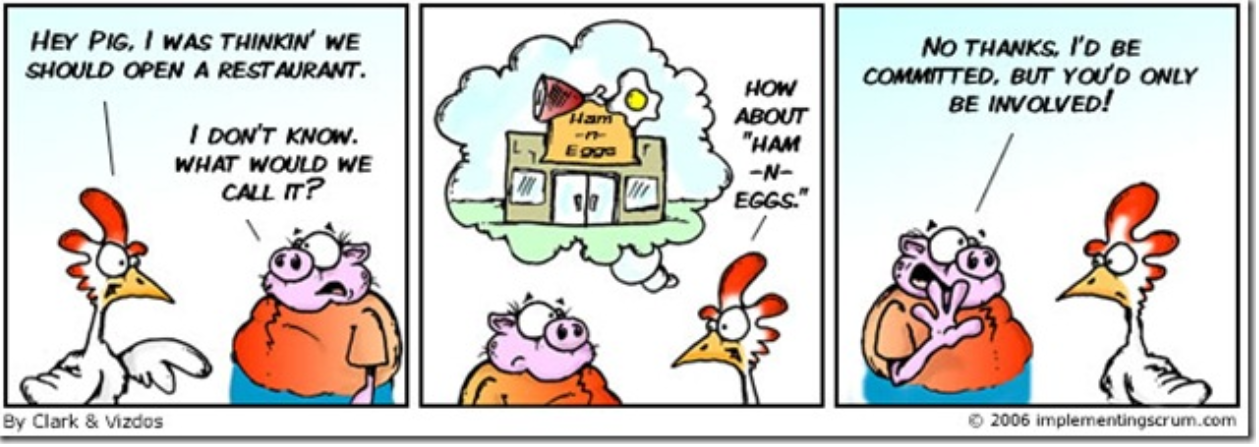
\includegraphics[width=0.8\textwidth]{chickenAndPig.png}
\end{center}

К основным (<<свиньям>>) относят три роли: product owner, scrum master и разработчик. Они полностью включены в проект и в Scrum-процесс, они создают продукт и отвечают за него деньгами и репутацией.

Вспомогательные роли (<<куры>>): пользователи, заказчики, HR, эксперты~--- разумеется, они тоже заинтересованы в проекте и даже расстроятся, если он загнётся, но степень их вовлечения и ответственности за проект ниже. Требования, пожелания, идеи и влияние <<кур>> принимаются во внимание, но все ключевые решения принимают всё равно <<свиньи>>.

\subsection{Product owner}

Product owner~--- это человек, который управляет видением проекта, управляет тем, куда этот проект движется. Как правило, это product manager для продуктовой разработки, менеджер проекта для внутренней разработки и представитель заказчика для заказной разработки. Он взаимодействует с командой и заказчиком и формулирует новые требования, отвечает за то, чтобы создаваемый продукт имел как можно больше пользы для бизнеса и пользователей. Сам Product owner в процессе разработки не участвует, но только он имеет право добавлять задачи в общий список задач, он же объясняет их разработчикам и отвечает и за приоритезацию задач. В конце каждой итерации он единственный, кто определяет, насколько успешно или неуспешно она закончилась.

Product owner~--- это единая точка принятия окончательных решений для команды в проекте, именно поэтому это всегда один человек, а не группа или комитет. И что еще более важно: он не должен совпадать со scrum мастером и с членами команды разработки. Это должен быть отдельно выделенный человек.

\subsection{Scrum master}

Scrum master~--- крайне важная роль. Он отвечает за успех внедрения Scrum в проекте, за то, чтобы Scrum-процесс шел правильно. Он следит за соблюдением всех правил, следит за тем, чтобы все было вовремя, чтобы все делали определенные вещи в установленное время и генерировали определенные артефакты. Scrum master формирует процесс, позволяющий эффективно организовать решение сложной проблемы или спорной ситуации, без потерь времени и сил выполнять все пункты совещаний (этот процесс еще называют фасилитацией) и т.п. Это что-то типа модератора, который за всеми следит со стороны и не допускает отклонений от хода процесса из-за эмоций, увлечённости техническими деталями или каких-то других отвлекающих факторов.

Scrum master является лидером, он всеми управляет, но на самом деле, никакой власти у него нет (т.е. лидер-слуга). Любой разработчик, если захочет, может ему не подчиняться. Он не может никого выгнать из команды. Но т.к. все высококвалифицированные, ответственные и объединены единой целью, то все его слушаются, поступают согласно его советам.

\subsection{Команда разработки}

Члены команды отвечают за разработку программного продукта. Размер команды ограничивается размером группы людей, способных эффективно взаимодействовать лицом к лицу. Типичный размер команды~--- 7 ± 2 человек.

Команда в Scrum кросс-функциональна. В нее входят люди с различными навыками, нет заранее определенных и поделенных ролей в команде, ограничивающих область действий членов команды. Опять же на всех членов команды распространяется коллективная ответственность. Не приветствуется, когда в вашей команде есть иерархия. Есть один только термин~--- разработчик. Даже если вы дизайнер, тестировщик~--- вы все равно разработчик. Все равны. Именно такая должна быть команда.

В связи с применяющимися практиками и совещаниями (см. ниже) оригинальный Scrum не очень хорошо дружит с распределёнными командами, хотя последнее время на эту тему появилось довольно много информации (см., например, \url{https://learn.microsoft.com/en-us/archive/msdn-magazine/2012/january/agile-development-working-with-agile-in-a-distributed-team-environment} (дата обращения: 04.03.2023)).

Как упоминалось выше, ни Product owner, ни Scrum master по сути напрямую не управляет командой. Команда самоорганизуется для выполнения задач и принимает все решения по разработке внутри себя.

\section{Product Backlog}

Самый главный артефакт в Scrum~--- Product Backlog. Это приоритезированный список имеющихся на данный момент задач по реализации проекта. В него помещается все, что нужно сделать в проекте. Не только бизнес- и технические требования, а вообще все: например, провести семинар, обучить пользователей, купить стол и т.п. Записывается то, что нужно сделать и затем все это оценивается некоторым количеством баллов: насколько задача сложная, сколько времени она займет и т.д.

Backlog постоянно пересматривается и дополняется: в него включаются новые требования, удаляются ненужные, пересматриваются приоритеты. За Product Backlog отвечает Product owner. Он единственный может туда что-то помещать и ставить приоритеты. Product owner отвечает за бизнес, команда~--- за техническую сторону. То есть Product owner добавляет задачи, команда их оценивает, а затем он может переупорядочить задачи в зависимости от их сложности.

Backlog~--- это артефакт, который живет в течение всего процесса выполнения. И если у вас есть несколько команд, которые разрабатывает один проект, он будет один для всех команд. Важно, что Product Backlog должен быть ориентирован на бизнес, т.е. на то, <<что надо>>, а не на то, <<как сделать>>.

Backlog может выглядеть совершенно по-разному. Может выглядеть, например, вот так:

\begin{center}
    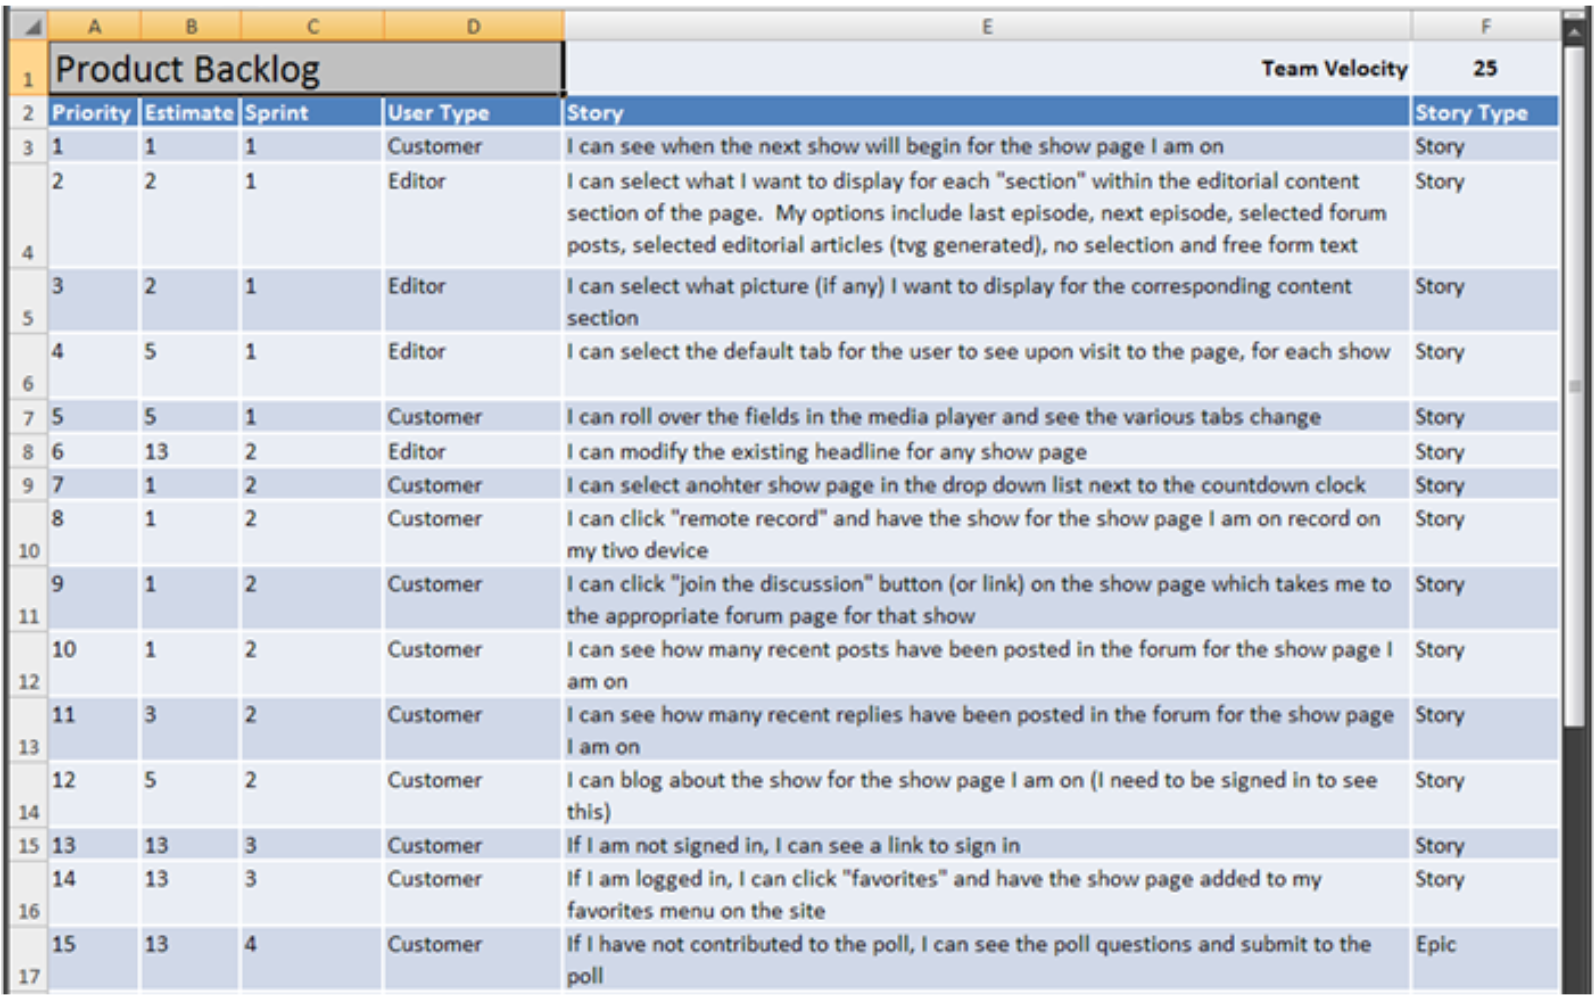
\includegraphics[width=0.9\textwidth]{backlog.png}
\end{center}

Обычно используется следующий формат: <<я как (роль), хочу (функциональность), для того, чтобы (цель)>>. Т.е. здесь сразу видно, на кого задача ориентирована, что надо делать и зачем это. На самом деле, это очень хороший формат, который заставляет сразу задуматься: <<зачем мы это делаем? Кому это надо?>> Это те два вопроса, над которыми программисты очень не любят думать, но над которыми думать очень полезно.

В принципе, в какой-то момент Backlog может стать пустым. Это означает, что проект закончен, и больше делать нечего, всё уже сделали. Нет ни багов, ни пожеланий. Но это крайне редкая ситуация.

\section{Спринты}

В Scrum итерация называется Sprint. Продолжительность спринта обычно составляет от одной недели до четырех. Очень часто используются неделя или две. По результатам каждого спринта получается некая рабочая версия, называемая инкрементом, которая реализует новые фичи.

Важно, что когда вы начали спринт, его состав работы <<замораживается>>. Элементы работы, включенные в очередной спринт, не подлежат изменению до его окончания. Если нужно добавить какие-то новые требования, которые нужно срочно сделать, то существует некая хитрая процедура добавления новой задачи во время работы спринта, но обычно так никто не делает и задачи просто помещаются в Product Backlog, возможно с высоким приоритетом, но всё равно на следующую итерацию.

Когда спринт заканчивается, происходят два события: ревью и ретроспектива. На них вы сидите и обсуждаете: что было хорошо, а что плохо. Поэтому удобно делать спринты недельными. В понедельник утром начинаете с планирования, а в пятницу вечером ретроспектива. Но кому-то недели оказывается мало, особенно с учётом всех плановых мероприятий, поэтому делают две или больше.

\subsection{Планирование спринта}

Планирование спринта~--- мероприятие, продолжительность которого зависит от частоты его проведения: в случае недельного~--- 2-3 часа, в случае месячного~--- чуть ли не целый день. На этом мероприятии происходит планирование задач, которые попадут в спринт: берётся Product backlog и начинают оценивать те задачи, которые являются самыми приоритетными. На основе отобранных задач формируется так называемый Sprint Backlog~--- TODO на ближайшую итерацию. Присутствуют Product owner, Scrum master и все разработчики.

Каждая задача оценивается не в днях, не в часах, а в некоторых поинтах. Обычно используют одну из следующих шкал: числа Фибоначчи (1, 2, 3, 5, 8, 13...), линейную шкалу (1, 2, 3, 4...), степени двойки (1, 2, 4, 8, ...), размеры одежды (XS, S, M, L...).

Как оценить задачу так, чтобы все приняли согласованное решение? Есть много разных практик оценивания. Одна из них~--- planning poker\footnote{см., например, \url{https://firepoker.io/} (дата обращения: 04.03.2023).}. Выглядит примерно так: заводятся специальные карточки, на которых написаны числа. Например: 1, 2, 3, 5, 8... Каждому участнику обсуждения выдаётся по одной колоде карт (в этом процессе оценивания участвуют только разработчики, Product owner наблюдает, Scrum master модерирует). Участники выбирают по одной карте и кладут их рубашкой вверх, показывая таким образом, что выбор сделан. Затем все эти карточки переворачиваются и сравниваются. (Таким образом, покер планирования минимизирует эффект привязки\footnote{https://ru.wikipedia.org/wiki/Эффект\_привязки (дата обращения: 04.03.2023).} путем опроса каждого из участников команды таким образом, что никто не знает чужого решения до одновременного оглашения выбора каждого из участников.) Участникам с различающимися оценками дается возможность высказаться и обосновать свой выбор. Таким образом происходит обмен информацией о задаче. После обсуждения проводится повторное голосование, и так до тех пор, пока не будет достигнут консенсус. Любая задача в ходе итерации может достаться любому разработчику, поэтому крайне важно, чтобы каждый чувствовал в себе уверенность выполнить задачу за то количество поинтов, за которое он голосует.

В конце каждого спринта подсчитывается количество поинтов задач, которое вы закрыли за этот спринт. Это так называемая скорость команды (team velocity)\footnote{Вспоминаем также коэффициент, на который умножали оценку задач в XP, тут без него тоже не обойтись.} Следовательно, зная среднее число поинтов за предыдущие спринты, вы можете примерно спрогнозировать, сколько вы сделаете за следующий спринт. Поэтому следует набирать столько задач, чтобы примерно набралось то среднее число поинтов плюс некоторый небольшой запас.

\subsection{Этап разработки}

В процессе работы над итерацией часто используются канбан-доски. Они  позволяют быстро оценить прогресс проекта, да и организовать их довольно просто (доступны также куча инструментов для организации досок онлайн, например, Trello или Pivotal Tracker). Даже GitHub умеет канбан-доску <<прямо из коробки>>, достаточно включить её в настройках репозитория:

\begin{center}
    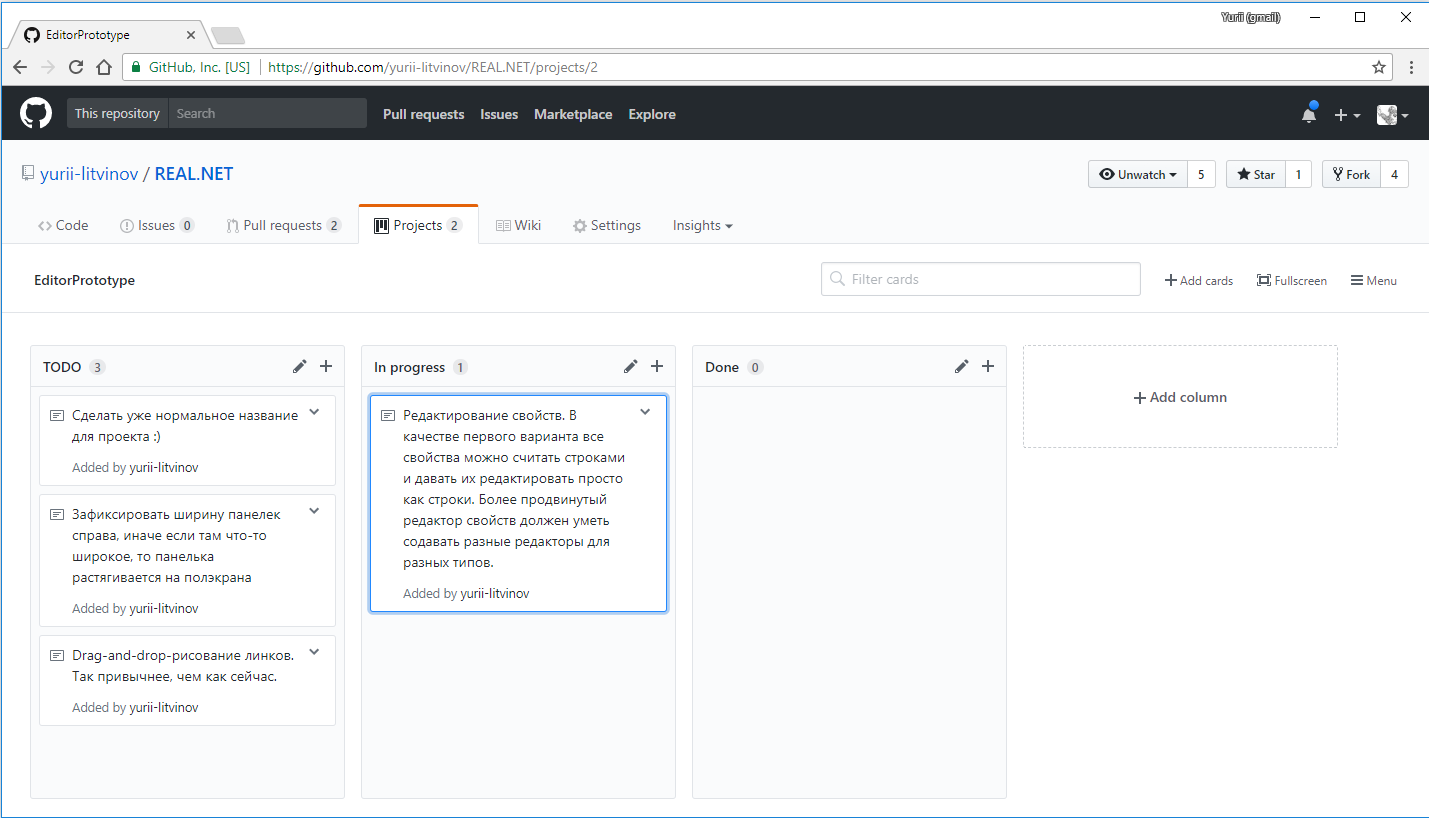
\includegraphics[width=\textwidth]{githubProjects.png}
\end{center}

Когда кто-то хочет взять новую задачу, то берёт свободную карточку из backlog’а и переклеивает ее в колонку work in progress. Если кто-то хотел делать эту задачу, но пришел и увидел, что она in progress~--- значит берет другую. Набор колонок может варьироваться, но наиболее распространены TODO, In progress и Done. Всё остальное~--- по необходимости. При желании также можно разбить эти колонки на строки по разработчикам, подсистемам или каким-то другим критериям.

Ещё есть крайне полезная вещь~--- диаграмма сгорания задач. Она показывает, сколько уже задач сделано и сколько ещё остаётся сделать в текущем спринте. Ее обычно держат где-то на видном месте поблизости с доской: 

\begin{center}
    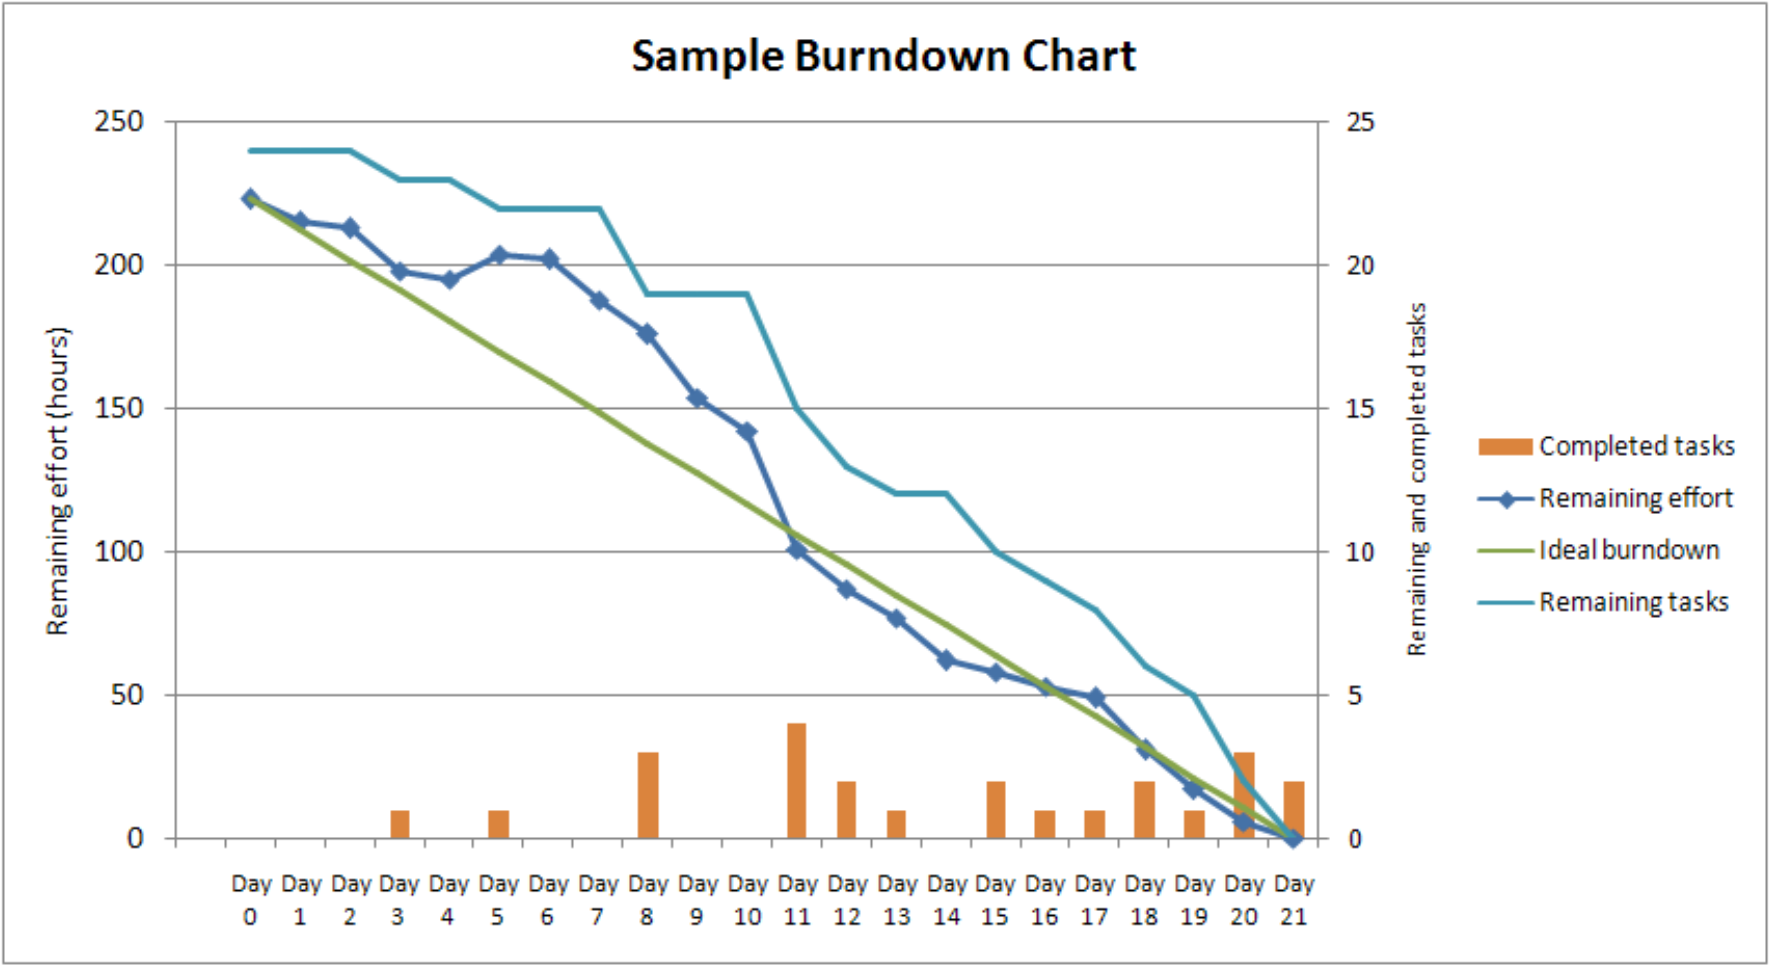
\includegraphics[width=0.9\textwidth]{burndownChart.png}
\end{center}

Рисуется сначала ориентир (прямая): как должен развиваться проект, чтобы всё успеть к дате завершения, если работать равномерно, и ничего не будет прибавляться и пропадать. Remaining effort~--- это сколько осталось сделать в часах, Remaining tasks~--- в задачах, бывает ещё кривая в поинтах. Чтобы не перегружать график, из них обычно рисуется что-то одно.

Обновление этого графика~--- ежедневная обязанность Scrum master’а. Если кривая долго не опускается вниз, это хороший повод задуматься и пересмотреть процесс и/или границы проекта.

Ещё стоит отметить, что нет персонального графика по каждому разработчику, есть только график на всю команду. Во-первых, команда предполагается более-менее равная, а во-вторых, ситуация, когда есть кто-то, кто делает сильно больше остальных, считается не очень хорошей. Если у него есть такой серьёзный перевес в знаниях, то будет гораздо лучше, чтобы он помогал набираться знаний остальным членам команды, тогда со временем все начнут работать более эффективно. На 100\% командная игра~--- либо все вместе выиграли, либо все вместе проиграли.

\subsection{Ежедневные встречи}

Ежедневные Scrum-собрания имеют продолжительность не более 15 минут. Это совещание проходит стоя как раз для того, чтобы собрание не затягивалось. Цель митинга~--- поделиться информацией. Происходит всегда в одно и то же время (никого не ждут), в одном и том же месте. Обязательно присутствуют все разработчики и Scrum master, Product owner по желанию или необходимости. На этом собрании каждый разработчик отвечает на 3 вопроса:

\begin{itemize}
    \item Что он сделал за сутки? 
    \item Что будет делать до следующего собрания?
    \item Какие у него есть проблемы? 
\end{itemize}

Но нужно понимать, что данное собрание не предназначено для решения проблем в проекте. Все требующие специального обсуждения вопросы должны быть вынесены за пределы митинга. Т.е. вы говорите о проблеме и потом, возможно, сразу же после этого собрания будет другое собрание, на котором останутся нужные люди и помогут вам в ваших вопросах.

Это собрание проводится для того, чтобы поддерживать некое общее понимание того, что вообще происходит. С одной стороны, это интересно, поскольку позволяет знать, кто и что делает. Но с другой стороны, некоторые могут рассказывать о тех вещах, до которых вам нет никакого дела: например, команда слишком большая и в ней начинают организовываться подкоманды по направлениям. Нужно следить за тем, чтобы люди на этих собраниях не вдавались в технические подробности, а лишь просто говорили о том, что происходит.

Есть еще такое мероприятие, как Scrum of scrums. Оно актуально, когда есть несколько Scrum-команд, работающих параллельно. Проводится оно после ежедневного scrum-совещания, и на него уже собираются только Scrum мастера этих команд (или технические специалисты, если собрание более технически ориентированное) и каждый говорит за всю свою команду. Каждый озвучивает ровно те же три вопроса плюс вопрос взаимодействия между командами, если с чем-то нужна сторонняя помощь. Это позволяет эффективно применять Scrum в больших проектах.

\subsection{Ревью спринта/демо}

В конце спринта происходит демо/ревью, на котором команда разработки показывает, что было сделано за спринт. На это собрание приглашаются все: представители заказчика, дизайнеры, тестировщики, ген. директор и все остальные, кто может быть заинтересован в развитии проекта. Это полезно, когда есть несколько команд разработчиков или ещё отдельно тестировщики, дизайнеры и т.д. Все показывают свой какой-то маленький кусочек и у всех появляется представление, что сделала та или иная команда. Также появляется обратная связь от пользователей, что может повлиять на приоритет задач на следующий спринт. 

Длительность демо~--- не более четырёх часов само собрание плюс не более двух часов на подготовку.

\subsection{Ретроспектива спринта}

Ретроспектива часто проводится сразу после демо. Но это уже более закрытая встреча, туда не пускают всех подряд. Ретроспектива является совещанием проектной команды в конце спринта с целью выявления удачных и неудачных действий за период с упором на то, что можно улучшить, выполняя последующие итерации. Помимо разработчиков обязательно присутствует Scrum-master. Длительность~--- 1-3 часа.

Итого, с учётом всего вышеперечисленного весь Scrum процесс можно описать следующей схемой:

\begin{center}
    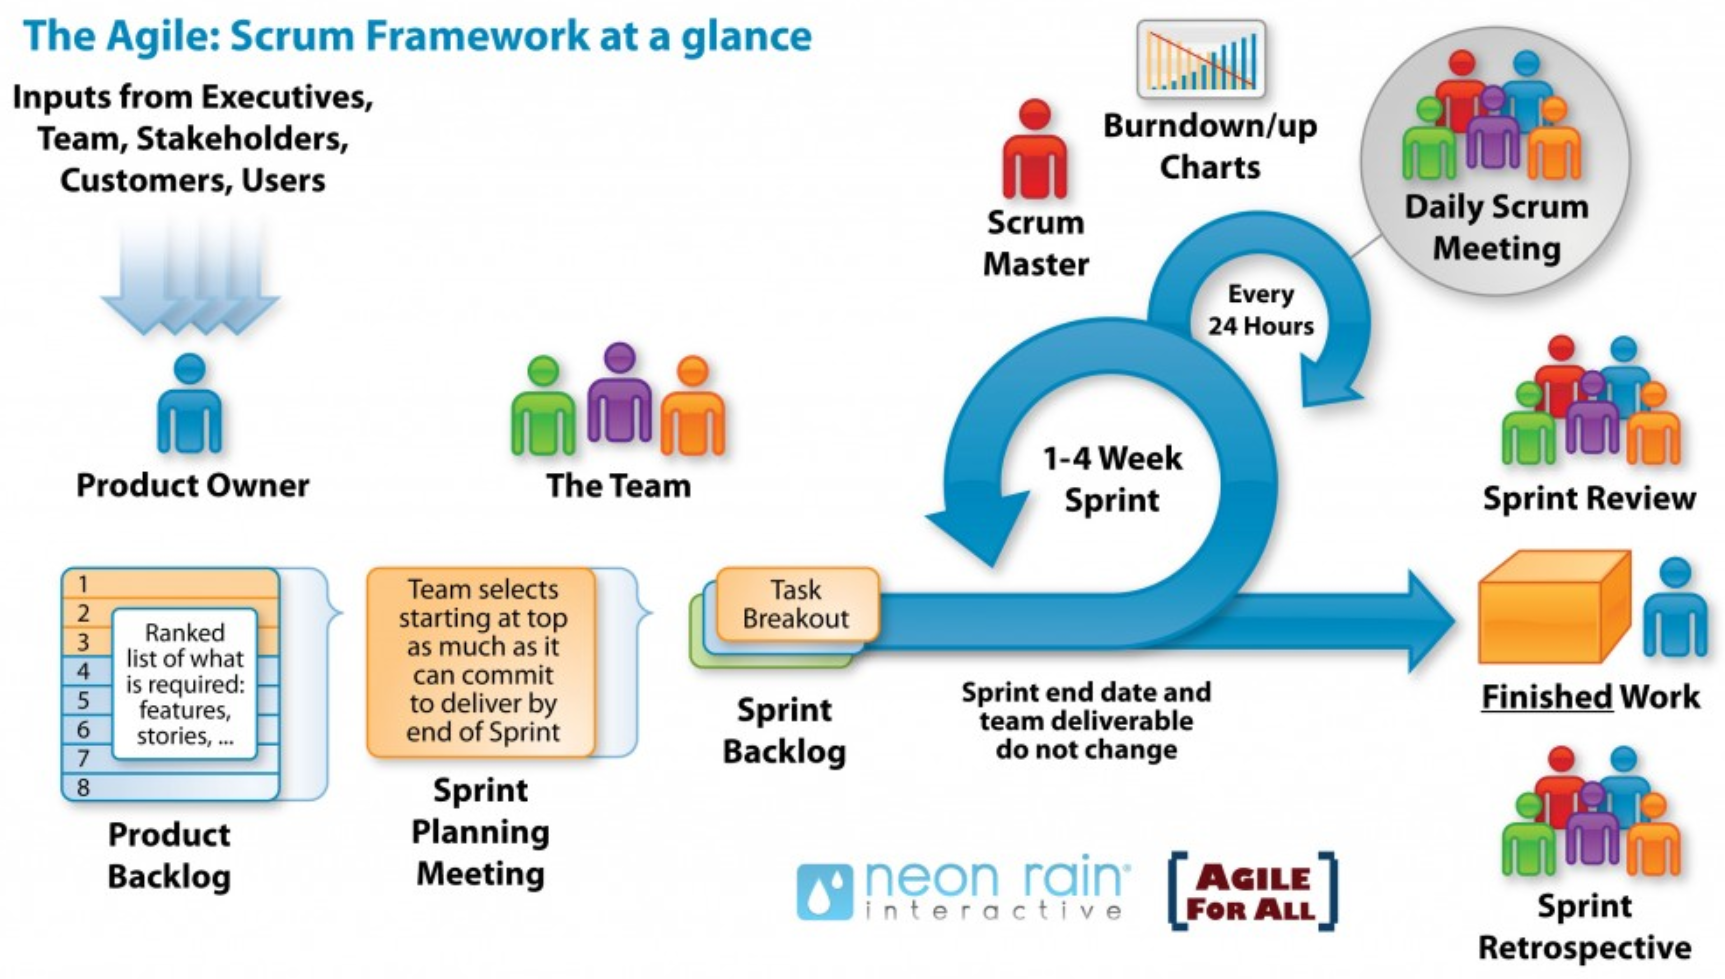
\includegraphics[width=0.9\textwidth]{scrumProcess.png}
\end{center}

\section{ScrumAnd (Scrum++)}

Есть два слова, которые обычно сравнивают со Scrum: ScrumAnd и ScrumBut. ScrumAnd означает, что вы делаете все согласно Scrum, но при этом добавляете еще какие-либо новшества. Например, есть популярная штука~--- нулевой спринт. Это как обычный спринт, по тем же правилам, но только в этот нулевой спринт занимаются проектированием и прототипированием, всю неделю. Понятно, что кучу диаграмм и большой набор диаграмм никто не делает, но подумать над архитектурой бывает полезно. Ещё примеры таких бонусов:

\begin{itemize}
    \item использование релевантных практик XP~--- многие практики из XP в Scrum применяются и так (например, короткие итерации, непрерывная интеграция), но если добавить Test-Driven Development или парное программирование, может стать лучше (а может и нет, это от проекта зависит);
    \item ревью кода~--- Scrum этого не требует, но это применяется повсеместно;
    \item высокий процент test/code coverage~--- тоже, не то чтобы секрет, очень многие проекты автоматизируют подсчёт тестового покрытия и имеют жёсткие правила по его минимуму;
    \item тестирование всей командой~--- Scrum и так предполагает кроссфункциональность, так что в команде не должно быть выделенного тестировщика, однако в дополнение к обычному тестированию можно проводить тест-фесты с призами за найденные баги, когда вся команда приостанавливает разработку и занимается только тестированием;
    \item недельные спринты~--- Scrum требует длительность спринта от недели до месяца, неделя удобнее всего, но страшнее всего для новичков;
    \item широкая аудитория на демо~--- не только команда и Product Owner, но и соседние команды, заказчик, потенциальные пользователи~--- все, кого смогли поймать;
    \item автоматизация~--- автоматизация всего, что только можно, это практика, популяризованная культурой DevOps, но Scrum + DevOps~--- это лучше, чем просто Scrum.
\end{itemize}

\section{ScrumBut(Scrum--)}

Под ScrumBut понимают, что вы используете Scrum, но при этом вам что-то могло не понравиться и вы решили это заменить на что-нибудь другое или вовсе вычеркнуть из списка. Нужно быть очень аккуратным, поскольку есть риск выкинуть что-то очень важное, и вся польза от Scrum в общем-то пропадет. Ниже приведены некоторые часто встречающиеся в индустрии примеры:

\begin{itemize}
    \item персонализация задач/спринтов/багов~--- это убивает командную ответственность и распределение знаний, делает бесполезным подход к планированию, изложенный выше, и банально приводит к простоям, когда на одного члена команды навалили вдвое больше работы, чем на остальных;
    \item <<водопад>> внутри спринта~--- последовательное прохождение фаз, когда все сначала проектируют, потом кодируют, потом тестируют, усложняет планирование в разы и делает практически невозможным релиз в конце спринта (наверняка что-то не успеют закодить или протестировать, а поскольку у нас водопад, то всё или ничего);
    \item ориентация на тулы вместо прямой коммуникации~--- частая мантра <<если это может быть письмом, не организуйте митинг>> в Scrum (да и вообще в Agile) не работает, потому что критически важна ширина канала обмена информацией; видеоконференции, как показывает практика, достаточно хороши, но командные чаты уже не вытягивают;
    \item 6-12-недельные спринты, перерывы между спринтами~--- например, перерыв на рефакторинг; убивает планирование (например, team velocity не посчитать), ухудшает цикл обратной связи;
    \item Big Design Up-Front (BDUF)~--- в Agile так не делают (хотя и не отрицается ценность архитектуры);
    \item отсутствие Scrum master’а~--- тогда процесс идёт как попало, никто не рисует Burndown Chart-ы, не следит за канбан-доской, не мотивирует разработчиков играть по правилам.
\end{itemize}

Вот ещё пара примеров:

\begin{center}
    \begin{tabularx}{\textwidth} { 
        | >{\centering\arraybackslash}X 
        | >{\centering\arraybackslash}X 
        | >{\centering\arraybackslash}X | }
        \hline
        ScrumBut                       & Причина                                           & Решение/Оправдание \\
        \hline
        Мы используем Scrum, \emph{НО} & Делать Daily Scrum для нас слишком накладно       & Daily Scrum будет только один раз в неделю               \\
        \hline
        Мы используем Scrum, \emph{НО} & Ретроспективы для нас~--- пустая трата времени    & Мы решили их не проводить                                \\
        \hline
        Мы используем Scrum, \emph{НО} & Мы не можем доставить инкремент продукта за месяц & Устанавливаем спринт длиной шесть недель                 \\
        \hline
        Мы используем Scrum, \emph{НО} & Иногда наши менеджеры дают специальные таски      & Готовые таски не всегда соответствуют Definition Of Done \\
        \hline
    \end{tabularx}
\end{center}

\subsection{Принцип Шу-Ха-Ри}

Есть такая практика изучения боевых искусств в Японии, согласно которой существует понятие о трёх ступенях:

\begin{itemize}
    \item Шу (соблюдать)~--- первым этапом вы просто повторяете за мастером то, что он делает, заучивая при этом технику, практику, движения.
    \item Ха (прорываться)~--- на втором этапе вы начинаете чувствовать и понимать, что стоит за этой техникой.
    \item Ри (отделяться)~--- на третьем этапе вы становитесь мастером. Вы знаете правила, можете делать изменения и осознавать их последствия. Вы сами себе ставите задачи и ищете возможности их реализации.
\end{itemize}

\begin{center}
    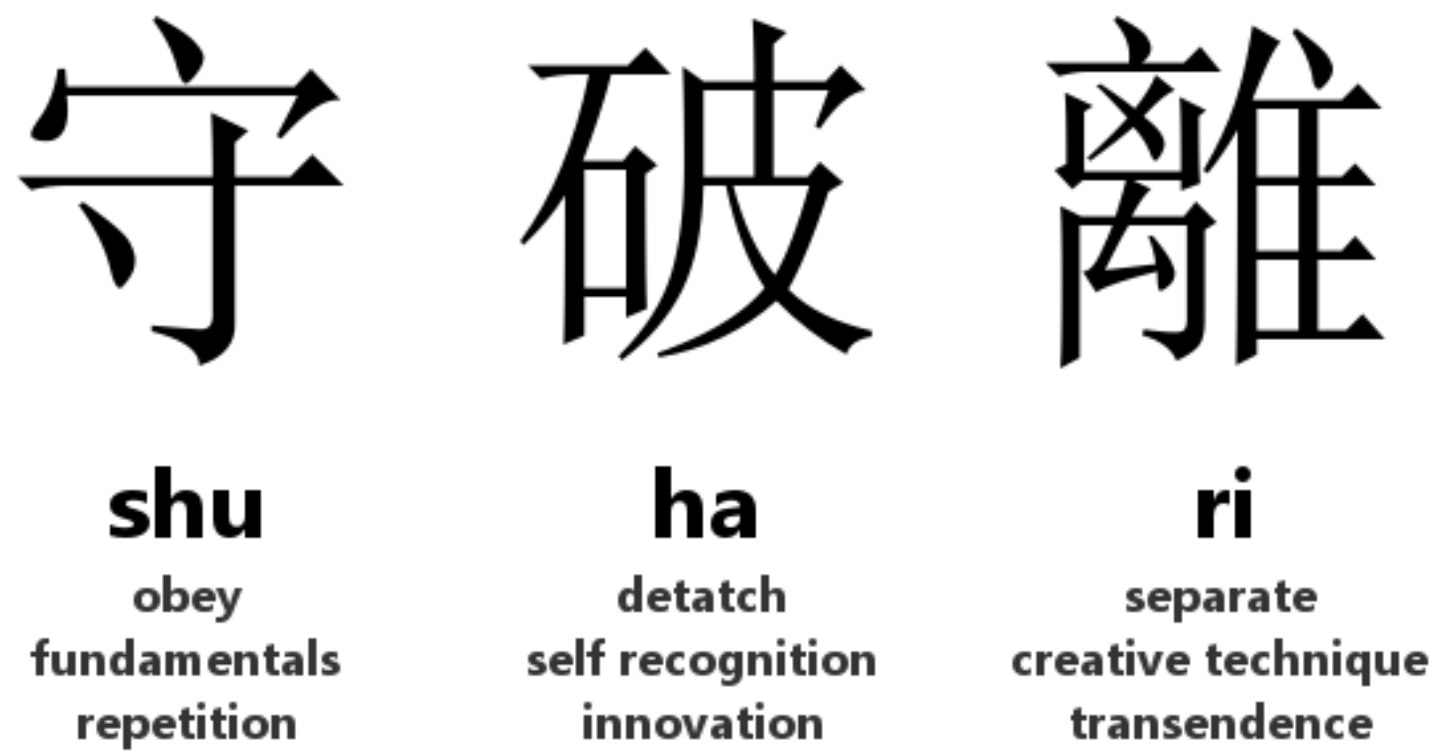
\includegraphics[width=0.7\textwidth]{shuHaRi.png}
\end{center}

Т.е. модифицировать процессы разработки надо только на третьем этапе, когда вы уже хорошо осознали, как и почему они работают. Иначе есть риск вносить изменения в технику, не понимая вещей, которые за ней стоят, и, как следствие, не получить нужного эффекта и закрепить неправильное представление о всей практике в целом. Нарушение этого принципа и приводит чаще всего к ScrumBut. 

\section{Ограничения Scrum}

\begin{itemize}
    \item fixed-cost/fixed-time проекты~--- как и вообще Agile; невозможно использовать преимущества гибкости, потому что стоимость/сроки зафиксированы и есть чёткое ТЗ;
    \item безответственные, низко мотивированные работники~--- в Scrum можно ничего не делать, просто задачи в следующий спринт перекладывать;
    \item слишком узкоспециализированные работники~--- им придётся назначать задачи в области их компетенции, и всё гибкое планирование, на котором стоит Scrum, развалится;
    \item неполноставочники~--- будут пропускать Daily Scrum, могут быть долго недоступны для общения, сложно планировать (и считать скорость команды);
    \item большое количество внешних зависимостей~--- убивает гибкое планирование;
    \item legacy или системы повышенной надежности~--- водопадные процессы лучше тут подходят: короткий цикл обратной связи хорошо работает только если у вас багрепорты~--- не экстренное сообщение в новостях о техногенной катастрофе;
    \item распределенные команды~--- в классической литературе по Scrum распределённость убивает коммуникации и обмен знаниями; в постковидном мире вполне научились работать распределённо. Однако команда должна быть в близких часовых поясах, иначе будут проблемы с Daily Scrum и прочими командными мероприятиями. Если так не получается, можно поделиться на несколько команд.
\end{itemize}

\end{document}
